\documentclass[minted]{codebook}
\usemintedstyle{tango}
\usepackage{tikz}
\usetikzlibrary{matrix}
\usepackage{lipsum}
\usepackage{biblatex}
\usepackage{graphicx}

\usepackage{tabularx}
\usepackage{siunitx}
\usepackage{multirow}

\newminted{tex}{}

\usepackage{makeidx}
\makeindex%[columns=2,intoc]
% \indexsetup{othercode=\small}

\begin{document}

\frontmatter

\author{Daniel Heck}
\title{Codebook}
\subtitle{A LaTeX Class for Technical Books}

\maketitle

\begin{copyrightpage}
Copyright \textcopyright{} 2021 by Daniel Heck

This work may be distributed and/or modified under the
conditions of the LaTeX Project Public License, either version 1.3
of this license or (at your option) any later version.
The latest version of this license is in
  \url{http://www.latex-project.org/lppl.txt}
and version 1.3 or later is part of all distributions of LaTeX
version 2005/12/01 or later.
\end{copyrightpage}


\begin{dedicationpage}
To me style is just the outside of content,\\
and content the inside of style,\\
like the outside and the inside of the human body---\\
both go together, they can't be separated.\par
\bigskip
\emph{Jean-Luc Godard}
\end{dedicationpage}


\tableofcontents

\chapter{Introduction}

\emph{Codebook} is a \LaTeX{} package for writing technical books,
especially books in computer science, mathematics, and related fields.
It is based on the standard \texttt{book} class, but it completely changes the design and layout and adds several new commands and environments for typesetting the following:
\begin{itemize}
  \item Copyright and dedication pages;
  \item Epigraphs at the beginning of a chapter;
  \item Exercises and solutions;
  \item Wide figures and tables that can reach into the margins;
  \item Code listings, either embedded into the text or floating;
  \item Predefined colors.
\end{itemize}
It is based on the standard \texttt{book} class so it should be compatible with most \LaTeX{} packages out there.

This class grew out of a set of macros and \LaTeX{} definitions I wrote for my personal book projects.
My goal was to support a modern design that looks good when printed on paper and when viewed as an eBook.
\emph{Codebook} uses three font families: the main text is set in \emph{Palatino}, headings in \emph{Source Sans Pro}, and source code \emph{Noto Mono Condensed}.
All three fonts are freely available and are included in current versions of \TeX{}live.

Visit \url{http://github.com/dheck/codebook} for the latest version.


\mainmatter

\part{Overview}

Parts are traditionally used to structure large documents into groups of related chapters.
For a small manual like this, parts are certainly overkill, but it allows you to see how they are formatted.
Notice that \emph{Codebook} allows you to include text after the title of a part, like here.


%--------------------------------------
\chapter{Writing Books using Codebook}
%--------------------------------------


Like any other \LaTeX{} document class, \emph{Codebook} is loaded using the \verb|\documentclass| command:
\begin{texcode}
\documentclass[options]{codebook}
\end{texcode}
The following options are supported:
\begin{itemize}
  \item \texttt{minted}: Loads the \texttt{minted} package and configures it to work well with \emph{Codebook}.
  \item \texttt{drafting}: Adds the current day to the footer and passes the option on to other packages that support it.
  Similar to the \verb|draft| option in the standard \LaTeX{} class this option is meant to be used while preparing the document and should be removed upon publication.
\end{itemize}



%--------------------------------------
\section{Formatting Text}
%--------------------------------------

Since \emph{Codebook} is based on the \verb|book| class, all standard \LaTeX{} commands and environments are supported, although many of them have been tweaked to fit the general design.
In addition, \emph{Codebook} provides several new commands and environments that are particularly useful in technical documents and textbooks.


\marginnote{Fonts and font sizes}
Different font sizes and can be selected using commands such as \verb|\tiny| and \verb|\large|;
an overview of all predefined font sizes is shown in Figure~\ref{fig:fontsizes}.
\begin{widetable}[htb]
  \small
  \caption{Predefined font sizes.}
  \label{fig:fontsizes}
  \begin{tabularx}{\textwidth}{lrX}
  \toprule
  \verb|\tiny| & 6\,pt & \tiny The quick brown fox\\
  \verb|\scriptsize| & 7\,pt & \scriptsize The quick brown fox\\
  \verb|\footnotesize| & 8\,pt & \footnotesize The quick brown fox\\
  \verb|\small| & 9\,pt & \small The quick brown fox\\
  \verb|\normalsize| & 10\,pt & \normalsize The quick brown fox\\
  \verb|\large| & 11.5\,pt & \large The quick brown fox\\
  \verb|\Large| & 13\,pt & \Large The quick brown fox\\
  \verb|\LARGE| & 15\,pt  & \LARGE The quick brown fox\\
  \verb|\huge|  & 20\,pt & \huge The quick brown fox\\
  \verb|\Huge|  & 24\,pt & \Huge The quick brown fox\\
  \verb|\HUGE|  & 30\,pt & \HUGE The quick brown fox\\
  \bottomrule
  \end{tabularx}
\end{widetable}


\marginnote{Predefined colors}
\emph{Codebook} defines a color palette you may want to use for highlighting text and for things like illustrations and code listings.
The full list of predefined colors is shown in Figure~\ref{fig:colors}.
In addition to the six basic colors \textcolor{cbBlue}{\texttt{cbBlue}}, \textcolor{cbGreen}{\texttt{cbGreen}}, \textcolor{cbRed}{\texttt{cbRed}}, \textcolor{cbOrange}{\texttt{cbOrange}}, \textcolor{cbYellow}{\texttt{cbYellow}}, \textcolor{cbBrown}{\texttt{cbBrown}}, and \textcolor{cbPurple}{\texttt{cbPurple}}, there are also six light variants like \textcolor{cbLightBlue}{\texttt{cbLightBlue}} and six dark variants like \textcolor{cbDarkRed}{\texttt{cbDarkRed}}.%
\footnote{The color palette is taken from the \emph{Tango Desktop Project}; see \url{https://en.wikipedia.org/wiki/Tango_Desktop_Project}}


\begin{figure}[htb]
  \centering
  \begin{tikzpicture}[nodes={minimum width=2.2cm,      
        text height=2.5ex,
        text depth=1.5ex,
        font=\ttfamily\small}]
    \matrix[matrix of nodes,column sep=4mm, row sep=4pt, inner sep=0pt, 
        column 2/.style={text=white},
        column 3/.style={text=white}
        ] {
      |[fill=cbLightBlue]| cbLightBlue & 
      |[fill=cbBlue]| cbBlue & 
      |[fill=cbDarkBlue]| cbDarkBlue
      \\
      |[fill=cbLightGreen]| cbLightGreen &
      |[fill=cbGreen]| cbGreen &
      |[fill=cbDarkGreen]| cbDarkGreen 
      \\
      |[fill=cbLightRed]| cbLightRed &
      |[fill=cbRed]| cbRed &
      |[fill=cbDarkRed]| cbDarkRed
      \\
      |[fill=cbLightOrange]| cbLightOrange &
      |[fill=cbOrange]| cbOrange &
      |[fill=cbDarkOrange]| cbDarkOrange 
      \\
      |[fill=cbLightYellow]| cbLightYellow &
      |[fill=cbYellow]| cbYellow &
      |[fill=cbDarkYellow]| cbDarkYellow 
      \\
      |[fill=cbLightBrown]| cbLightBrown &
      |[fill=cbBrown]| cbBrown &
      |[fill=cbDarkBrown]| cbDarkBrown
      \\
      |[fill=cbLightPurple]| cbLightPurple &
      |[fill=cbPurple]| cbPurple &
      |[fill=cbDarkPurple]| cbDarkPurple
      \\
    };
  \end{tikzpicture}
  \caption{Predefined colors.}
  \label{fig:colors}
\end{figure}



%--------------------------------------
\subsection{Notes}
%--------------------------------------

\emph{Codebook} provides several ways to add notes and supplementary information to the text.
As in all \LaTeX{} classes, you can add footnotes\footnote{Like this one.} using the \verb|\footnote| command.
Footnotes are tucked away at the bottom of the page and are therefore (by design!) easy to ignore.
Use them for information that is truly optional, or for information that you only include for the sake of completeness.

\marginnote{The \texttt{note} environment}
To include notes inside the running text, use the ``\texttt{note}'' environment:
\begin{texcode}
\begin{note}
Beware of bugs in the above code;
I have only proved it correct, not tried it.
\end{note}
\end{texcode}
This produces the following output:
\begin{note}
Beware of bugs in the above code;
I have only proved it correct, not tried it.
\end{note}
Since notes are visually set off from the main text it's clear that they provide supplementary information.
They are best used for information that every reader should aware of but that can be safely skimmed.

\marginnote{Margin notes}
Supplementary information that you want readers should be aware of, even if they don't need to understand all details, us \verb|\marginnote| command:
\begin{texcode}
\marginnote{Margin notes}
\end{texcode}
This example produces the margin note shown at the start of this paragraph.
Margin notes generally serve a different purpose than notes embedded in the text and footnotes:
They contain information that helps the reader, for example by summarizing the main points of a paragraph or group of paragraphs or by visually dividing a section into smaller pieces.

\marginnote{Boxes}
Finally, the \verb|aside| environment can be used to present information that is only indirectly related to the contents of the text.
For example, Box~\ref{box:urls} on page~\pageref{box:urls} describes a way to use footnotes for representing hyperlinks in documents that are meant to be printed \emph{and} read electronically.

\begin{aside}{Typesetting Hyperlinks}
\label{box:urls}
A common problem when writing technical documents is dealing with links to websites and other online resources.
Using \href{https://en.wikipedia.org/wiki/Hyperlink}{hyperlinks} is usually the best solution for electronic documents;
in \LaTeX{} this can be done using the \verb|\href| command from the \verb|hyperref| package.

In documents that are also meant to be printed and read offline, hyperlinks are not useful because the URL is invisible.
There are two better solutions.
If the web page is considered a primary or secondary source, add it to the bibliography and cite it like a book or an article \cite{wikipedia:hyperlink}.
Otherwise, simply use a \href{https://en.wikipedia.org/wiki/Hyperlink}{hyperlink}\footnote{\url{https://en.wikipedia.org/wiki/Hyperlink}} followed by a footnote that contains the URL.
\end{aside}



%--------------------------------------
\subsection{Code and Listings}
%--------------------------------------

For code and verbatim text, \emph{codebook} loads and configures the \emph{fancyvrb} package.
\begin{texcode}
\begin{Verbatim}
verbatim text
\end{Verbatim}
\end{texcode}
produces
\begin{Verbatim}
verbatim text
\end{Verbatim}
If you look closely, you will notice that verbatim blocks use a slighly smaller font size than \Verb|verbatim text| inside a paragraph.
Code inside \verb|Verbatim| environments is indented to distinguish it from the surrounding text.


In addition, \emph{codebook} provides two environments for longer listings that can float, similar to figures and tables.
The first environment is called \verb|listing|:
\begin{lst*}{The \texttt{listing} environment}
\begin{texcode}
\begin{listing}[htb]
...
\caption{...}
\label{...}
\end{listing}
\end{texcode}
\end{lst*}
As with other floats, you can influence the positioning of a particular listing by specifying location specifiers;
the default is ``\texttt{[tbp]}''.

\begin{listing}
\begin{Verbatim}
public class HelloWorld {
  public static void main(String[] args) {
    System.out.println("Hello World!");
  }
}
\end{Verbatim}
\caption{Hello world in Java.}
\label{lst:example}
\end{listing}

\begin{note}
By default, the \texttt{listing} environment sets up \texttt{fancyvrb} to draw thin lines above and below the code, as illustrated in Listing~\ref{lst:example}.
Packages that are based in \emph{fancyvrb} automatically work correctly;
Other \LaTeX{} packages for displaying code such as \emph{lstlisting} provide their own formatting options and must be configured by hand.
\end{note}

\marginnote{The \texttt{lst} and \texttt{lst*} environments.}
The second environment for embedding code listings is called \verb|lst|.
Unlike the normal \verb|listing| environment, \verb|lst|s don't float and are embedded in the surrounding text, similar to the way \verb|equation| or \verb|itemize| can occur in the middle of a normal paragraph.
In addition, code enclosed in a \verb|lst| environment can be broken across pages.
Code listings in \verb|lst| environments are numbered and have a caption, which must be specified as a mandatory argument.
In addition, a label can be specified as an optional argument, as in the following example:
\begin{texcode}
\begin{lst}[lst:hellopython]{Hello World in Python.}
\begin{Verbatim}
print("Hello World")
\end{Verbatim}
\end{lst}
\end{texcode}
Here, the label is \verb|lst:hellopython| and the caption \verb|Hello World in Python.|.
The listing is typeset as follows:
\begin{lst}[lst:hellopython]{Hello World in Python.}
\begin{Verbatim}
print("Hello World")
\end{Verbatim}
\end{lst}
The number of the listing and its caption are shown in the margin.

Alternatively, you can use the \verb|lst*| environment to produce an unnumbered listing:
\begin{texcode}
\begin{lst*}{Hello World in Python.}
\begin{Verbatim}
print("Hello World")
\end{Verbatim}
\end{lst*}
\end{texcode}
Since \verb|lst*| is unnumbered it doesn't take the label as an optional argument, and it doesn't output a number in front of the caption.




\begin{note}
The \texttt{minted} package defines its own \verb|listing| environment that conflicts with the one provided by \emph{Codebook}.
To use \texttt{minted}, you can load the \emph{Codebook} class as follows:
\begin{texcode}
\PassOptionsToPackage{optionlist}{minted}
\documentclass[minted]{codebook}
\end{texcode}
\end{note}


%--------------------------------------
\subsection{Exercises and Solutions}
%--------------------------------------

\emph{Codebook} provides an easy way to typeset exercises and their solutions.
Exercises are enclosed in the \verb|exercise| environment which takes an optional argument that includes a title.
Inside each exercise you can use the \verb|answer| environment to specify a solution.
The following example specifies a single exercise and its solution:
\begin{lst*}{Specifying exercises and their solutions.}
\begin{texcode}
\begin{exercise}[Typesetting formulas]
\label{ex:binomial}
Explain how to typeset the following formulas in \LaTeX{}:
\begin{tasks}
  \item $(x+y)^2=x^2 + 2xy + y^2$;
  \item $e^{i\pi}=-1$.
\end{tasks}

\begin{answer}
\begin{tasks}
  \item \verb|$(x+y)^2=x^2 + 2xy + y^2$|
  \item \verb|$e^{i\pi}=-1$|
\end{tasks}
\end{answer}
\end{exercise}
\end{texcode}
\end{lst*}
The \texttt{tasks} environment used in the example above behaves like \verb|itemize|, except that it uses alphabetic labels.
At the point in the document where the \verb|exercise| environment appears, only the exercise itself is printed:
\begin{exercise}[Typesetting formulas]
\label{ex:binomial}
Explain how to typeset the following formulas in \LaTeX{}:
\begin{tasks}
  \item $(x+y)^2=x^2 + 2xy + y^2$;
  \item \label{task:euler} $e^{i\pi}=-1$.
\end{tasks}

\begin{answer}
\begin{tasks}
  \item \verb|$(x+y)^2=x^2 + 2xy + y^2$|
  \item \verb|$e^{i\pi}=-1$|
\end{tasks}
\end{answer}
\end{exercise}
You can refer to exercises and tasks by labeling them as shown in the previous example. 
The label of an exercise contains both the number of the chapter and the exercise, so writing \verb|Exercise~\ref{ex:binomial}| produces ``Exercise~\ref{ex:binomial}.'' 
The label of a task contains just its alphabetic tag, so \verb|Task~\ref{task:euler}| produces ``Task~\ref{task:euler}.''

\marginnote{Loading answers}
The answers are not typeset immediately but saved to a separate file.
You can load all answers defined in the current document using the \verb|\inputanswers| command:
\begin{lst*}{}
\begin{minted}{tex}
\inputanswers
\end{minted}
\end{lst*}
This command outputs the \verb|answer|s of all exercises that were encountered so far.
For the single exercise defined above, \verb|\inputanswers| produces the following output:
\inputanswers

What if you want to print the answers output by one \LaTeX{} document in another document, for example when producing a separate solutions manual?
Since the lines in an \verb|answer| environment are simply written to a file called ``\verb|\jobname.solution|,'' where the macro \verb|\jobname| is the name of the current document, you can include the answers from a different \LaTeX{} document using the \verb|\input| or \verb|\include| commands.
For example, the answers defined in a document called \verb|myboook.tex| can be loaded in another document as follows:
\begin{texcode}
\input{mybook.solution}
\end{texcode}


%--------------------------------------
\subsection{Epigraphs}
%--------------------------------------

\begin{epigraphs}
\epigraph[\textsc{Terry Pratchett}, \emph{Hogfather}]
  {Real stupidity beats artificial intelligence every time.}
\end{epigraphs}

\noindent Many nonfiction books start each chapter with an \emph{epigraph},
an inspirational or humorous quote that fits the theme of the chapter.
To typeset such epigraphs, \emph{Codebook} provides the \verb|epigraphs| environment that can contain one or more \verb|\epigraph| commands.
The following example shows how the quote at the beginning of this subsection was specified:
\begin{texcode}
\begin{epigraphs}
\epigraph[\textsc{Terry Pratchett}, \emph{Hogfather}]
  {Real stupidity beats artificial intelligence every time.}
\end{epigraphs}
\noindent Many nonfiction books start each chapter with an \emph{epigraph},
\end{texcode}
The \verb|\noindent| command at the beginning of the first paragraph prevents \LaTeX{} from indenting the first line after the quote.

The following parameters determine the layout of epigraphs:
\begin{itemize}
  \item \verb|\epigraphwidth| (default: 3\,in). The width of the box that contains each epigraph.

  \item \verb|\beforepigraphskip| (default: 0\,in). The amount of space to insert before the \verb|epigraphs| environment.

  \item \verb|\afterepigraphskip| (default: 2\,pc). The amount of space to insert after the \verb|epigraphs| environment.
\end{itemize}
The values of these parameters can be changed using the \verb|\setlength| command.

%--------------------------------------
\section{Floating Material}
%--------------------------------------

%--------------------------------------
\subsection{Figures}
%--------------------------------------

In addition to the standard \texttt{figure} environment, \emph{Codebook} provides a \texttt{widefigure} environment that stretches across the entire width of the page.
An example of the standard \texttt{figure} environment is shown in Figure~\ref{fig:normal}.
Notice that captions are centered, so the contents of the figure should usually be centered as well.

\begin{figure}
  \centering
  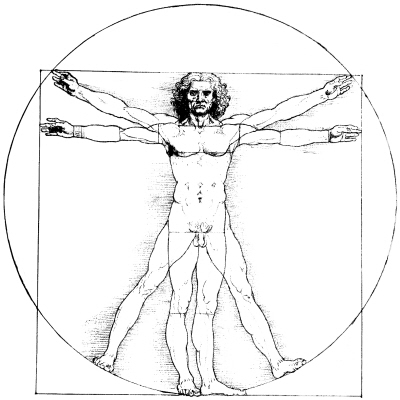
\includegraphics[width=2.5in]{vitruvian}
  \caption{A normal figure with a centered caption.}
  \label{fig:normal}
\end{figure}

For presenting images or other material that is wider than the body of the page, you can use the \texttt{widefigure} environment that extends into the margin of the page:
\begin{texcode}
\begin{widefigure}
  
\includegraphics[width=\fulltextwidth]{mandel-wide.png}
  \caption{A wide figure.}
\end{widefigure}
\end{texcode}
The result is shown in Figure~\ref{fig:wide}: it looks like a normal \texttt{figure} with the caption under the image, but it extends across the text block plus the margin area.
The length \verb|\fulltextwidth| used in the example above is defined by \emph{Codebook} as the width of the body plus the width of the margin.

\begin{widefigure}
  \centering
  
\includegraphics[width=\fulltextwidth]{mandel-wide.png}
  \caption{A wide figure.}
  \label{fig:wide}
\end{widefigure}


%--------------------------------------
\subsection{Tables}
%--------------------------------------

Table~\ref{tab:quarks} illustrates the recommended visual appearance of tables in \emph{Codebook}


\begin{itemize}
  \item The \verb|\caption| should come before the body of the table.
  \item The \verb|booktabs| package is used to draw horizontal rules.
\end{itemize}

\begin{table}
  \centering\small
  \caption{Quarks}
  \label{tab:quarks}
  \begin{tabular}{cccccS[separate-uncertainty=true]}
  \toprule
    \textbf{Generation} & \textbf{Name} & \textbf{Symbol} & \textbf{Spin} & \textbf{Charge [e]} & \textbf{Mass [MeV/c$^2$]} \\
  \midrule
     \multirow{2}{*}{1} & up      & u & $1/2$ & $+2/3$ & 2.2 +- 0.6\\
       & down    & d & $1/2$ & $-1/3$ & 4.6 +- 0.5\\
  \midrule
     \multirow{2}{*}{2} & charm   & c & $1/2$ & $+2/3$ & 1280 +- 30\\
       & strange & s & $1/2$ & $-1/3$ & 96(8)\\
   \midrule
     \multirow{2}{*}{3} & top     & t & $1/2$ & $+2/3$ & 173100(600)\\
       & bottom  & b & $1/2$ & $-1/3$ & 4180 +- 40\\
   \bottomrule
  \end{tabular}
\end{table}

The recommended way of formatting tables is to use the \texttt{booktabs} package, which is loaded automatically.
For example, Table~\ref{tab:quarks} is typeset as follows
\begin{texcode}
\begin{table}
  \centering\small
  \caption{Quarks}
  \label{tab:quarks}
  \begin{tabular}{cccccS[separate-uncertainty=true]}
  \toprule
    \textbf{Generation} & \textbf{Name} & \textbf{Symbol} & \textbf{Spin} & \textbf{Charge [e]} & \textbf{Mass [MeV/c$^2$]} \\
  \midrule
     \multirow{2}{*}{1} & up      & u & $1/2$ & $+2/3$ & 2.2 +- 0.6\\
       & down    & d & $1/2$ & $-1/3$ & 4.6 +- 0.5\\
  \midrule
    ...
  \bottomrule
  \end{tabular}
\end{table}
\end{texcode}
(This example relies on two additional packages that aren't loaded by \emph{Codebook}: the \texttt{siunitx} package for formatting columns of numerical data and the \texttt{multirow} package for the \verb|\multirow| command.)

\appendix

% \nocite{*}

\backmatter
% \printbibliography[heading=bibintoc]

\printindex

\end{document}